\documentclass{standalone}
\usepackage{tkz-graph}
\usetikzlibrary{arrows,graphs,matrix,positioning, arrows.meta}



\begin{document}
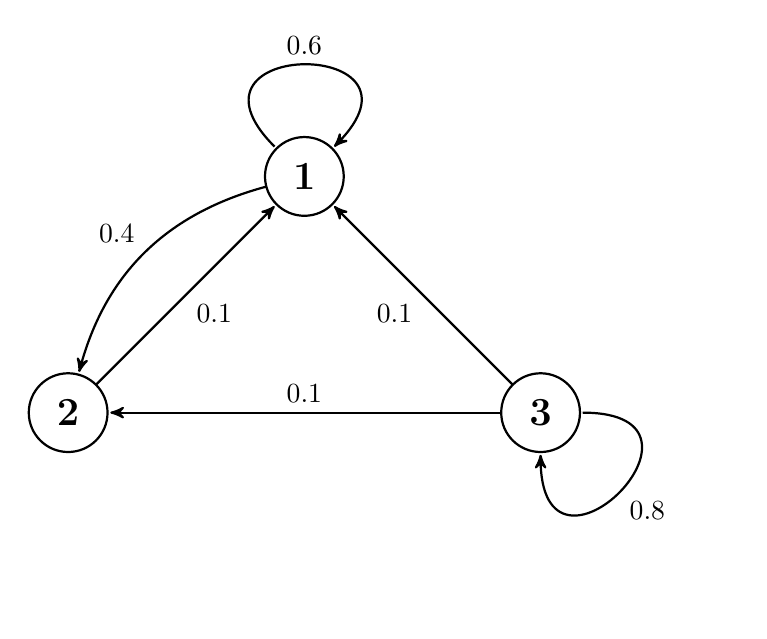
\begin{tikzpicture}[->,>=stealth',shorten >=1pt,thick]
\SetGraphUnit{3} 
\tikzset{VertexStyle/.style = {draw,circle, thick,
                               minimum size=1cm,
                               font=\Large\bfseries},thick} 
\Vertex{1} \SOWE(1){2} \SOEA(1){3} 
\Edges(3,2,1) \Edge(3)(1)

\Loop[dist=2cm,dir=NO,label=$0.6$,labelstyle=above](1)  
\Loop[dist=2cm,dir=SOEA,label=$0.8$,labelstyle=below right](3)  

\path[every node/.style={swap,auto}]    (2) to node {0.1} (1)
                                            to node {0.1} (3)
                                            to node {0.1} (2); 
\draw[->] (1) to [bend right] node [above left] {0.4} (2);
% it's possible with \Edge but Tikz's syntax is allowed too.
\end{tikzpicture} 



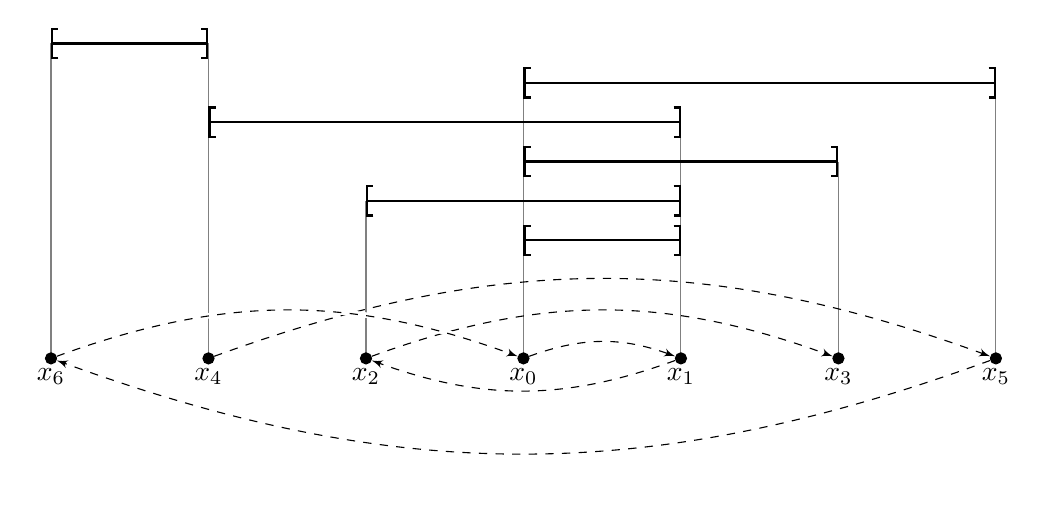
\begin{tikzpicture}

\tikzset{vertex/.style = {shape=circle, fill=black,draw,minimum size=4pt, inner sep=0pt}}
\tikzset{edge/.style = {->,> = latex'}}
\tikzset{interval/.style = {<->,> = {Bracket[length=0.8mm, width=4mm]}, line width = 0.8pt}}

%help lines
\draw[gray] (0, 0) -- (0, 4);
\draw[gray] (2, 0) -- (2, 4);
\draw[gray] (4, 0) -- (4, 2);
\draw[gray] (6, 0) -- (6, 3.5);
\draw[gray] (8, 0) -- (8, 3);
\draw[gray] (10, 0) -- (10, 2.5);
\draw[gray] (12, 0) -- (12, 3.5);
% vertices
\node[vertex] (1) at  (0, 0) {};
\node[vertex] (2) at  (2, 0) {};
\node[vertex] (3) at  (4, 0) {};
\node[vertex] (4) at  (6, 0) {};
\node[vertex] (5) at (8, 0) {};
\node[vertex] (6) at (10, 0) {};
\node[vertex] (7) at (12, 0) {};

\node[below] at (0, 0) {$x_6$};
\node[below] at (2, 0) {$x_4$};
\node[below] at (4, 0) {$x_2$};
\node[below] at (6, 0) {$x_0$};
\node[below] at (8, 0) {$x_1$};
\node[below] at (10, 0) {$x_3$};
\node[below] at (12, 0) {$x_5$};

%edges
\draw[edge, dashed] (4) to[bend left=20] (5);
\draw[edge, dashed] (5) to[bend left=20] (3);
\draw[edge, dashed] (3) to[bend left=20] (6);
\draw[edge, dashed] (2) to[bend left=20] (7);
\draw[edge, dashed] (7) to[bend left=20] (1);
\draw[edge, white, line width = 2pt] (1) to[bend left=20] (4);
\draw[edge, dashed] (1) to[bend left=20] (4);

%intervals
\draw[interval] (6, 1.5) -- (8, 1.5);
\draw[interval] (4, 2) -- (8, 2);
\draw[interval] (6, 2.5) -- (10, 2.5);
\draw[interval] (2, 3) -- (8, 3);
\draw[interval] (6, 3.5) -- (12, 3.5);
\draw[interval] (0, 4) -- (2, 4);

%\Loop[dist=1cm,dir=NO,label=$$,labelstyle=above](1)  

%\draw[edge, dashed] (2)  to[bend right] (3);
%\draw[edge] (6) to[bend left] (4);

%\draw[edge] (1) to[bend left] (2);
%\draw[edge] (2) to[bend left] (1);

%\path (a2) to node {\dots} (c);
%\node [shape=circle,minimum size=1.5em] (a3) at (4.5,0) {};
%\draw[edge] (a2) to[bend left] (a3);
%\draw[edge] (a3) to[bend left] (a2);

%\node [shape=circle,minimum size=1.5em] (c1) at (6.5,0) {};
%\draw[edge] (c) to[bend left] (c1);
%\draw[edge] (c1) to[bend left] (c);
\end{tikzpicture}

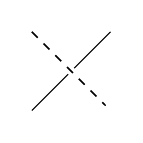
\begin{tikzpicture}
\draw (0,0) -- (1,1);
\draw[draw=white,double = black,very thick, dashed, ->] (0,1) -- (1,0);
\end{tikzpicture}

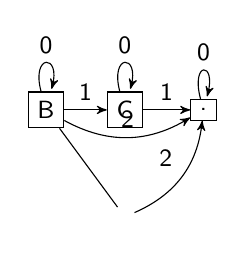
\begin{tikzpicture}[>=stealth',
    font=\sffamily\small,
    every node/.style={align=center},
    skip loop left/.style={to path={-- ++(-#1,0)|- (\tikztotarget)}},
    skip loop right/.style={to path={-- ++(#1,0)|- (\tikztotarget)}},
    hv path/.style ={to path={-| (\tikztotarget)}},
   vh path/.style ={to path={|- (\tikztotarget)}},
]
\node[draw] (root) {{.}};
\node[draw, left of=root] (C) {{C}} ;
\node[below=of C] (bC) {};
\node[draw, left of=C] (B) {{B}} ;
\graph[use existing nodes] {
 root->[edge label=0, loop above]root;
 C->[edge label=1]root;
 C->[edge label=0, loop above]C;
 B->[edge label=0, loop above]B;
 B->[edge label=1]C;
 B--bC->[edge label=2, bend right]root;
B->[edge label=2, bend right]root;
};
\end{tikzpicture}



\end{document} 